\subsection{两个平面垂直的判定和性质}\label{subsec:1-15}

两个平面相交,如果所成的二面角是直二面角,就说\zhongdian{这两个平面互相垂直}。

两个互相垂直的平面,画成如图 \ref{fig:ltjh-1-48} 那样。把直立平面的竖边画成和水平平面的横边垂直。
平面 $\alpha$ 和 $\beta$ 垂直,记作 $\alpha \perp \beta$。

\begin{figure}[htbp]
    \centering
    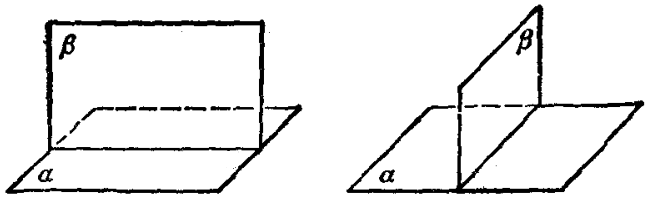
\includegraphics[width=9cm]{../pic/ltjh-ch1-48.png}
    \caption{}\label{fig:ltjh-1-48}
\end{figure}

判定两个平面垂直,有下面的定理:

\begin{dingli}[两个平面垂直的判定定理][dl:lgpmcz-pd]
    如果一个平面经过另一个平面的一条垂线,那么这两个平面互相垂直。
\end{dingli}

已知: $AB \perp \beta$, $AB \cap \beta =B$, $AB \subset \alpha$ (图 \ref{fig:ltjh-1-49})。

求证:$\alpha \perp \beta$。

证明:设 $\alpha \cap \beta = CD$,则 $B \in CD$。

$\because$ \quad $AB \perp \beta$, $CD \subset \beta$,

$\therefore$ \quad $AB \perp CD$。

在平面 $\beta$ 内过点 $B$ 作直线 $BE \perp CD$。
则 $\angle ABE$ 是二面角 $\alpha{-}CD{-}\beta$ 的平面角,又 $AB \perp BE$。\\
即 \quad 二面角 $\alpha{-}CD{-}\beta$ 是直二面角。

$\therefore$ \quad $\alpha \perp \beta$。

\begin{figure}[htbp]
    \centering
    \begin{minipage}[b]{7cm}
        \centering
        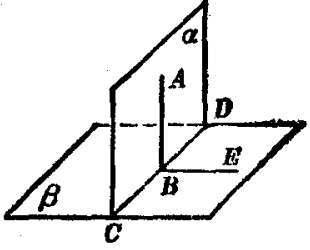
\includegraphics[width=5cm]{../pic/ltjh-ch1-49.png}
        \caption{}\label{fig:ltjh-1-49}
    \end{minipage}
    \qquad
    \begin{minipage}[b]{7cm}
        \centering
        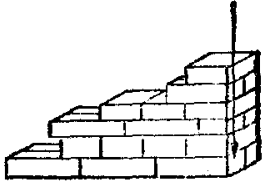
\includegraphics[width=5cm]{../pic/ltjh-ch1-50.png}
        \caption{}\label{fig:ltjh-1-50}
    \end{minipage}
\end{figure}

建筑工人在砌墙时,常用一端系有铅锤的线来检查所砌的墙面是否和水平面垂直(图 \ref{fig:ltjh-1-50})。
实际上,就是依据这个定理。

下面我们研究两个平面垂直的性质。

设平面 $\alpha$ 和 $\beta$ 垂直,它们交于直线 $CD$,平面 $\alpha$ 内的直线 $AB$ 垂直于 $CD$(图 \ref{fig:ltjh-1-49})。
我们看 $AB$ 是否垂直于平面 $\beta$。

在平面 $\beta$ 上引直线 $BE \perp CD$。 则 $\angle ABE$ 是二面角 $\alpha{-}CD{-}\beta$ 的平面角。

$\because$ \quad $\alpha \perp \beta$,

$\therefore$ \quad $AB \perp BE$。

又 $\because$ \quad $AB \perp CD$,

$\therefore$ \quad $AB \perp \beta$。

由此我们得到下面的定理:

\begin{dingli}[两个平面垂直的性质定理][dl:lgpmcz-xz]
    如果两个平面垂直,那么在一个平面内垂直于它们交线的直线垂直于另一个平面。
\end{dingli}




\liti \zhongdian{如果两个平面互相垂直,那么经过第一个平面内的一点垂直于第二个平面的直线,在第一个平面内。}

已知: $\alpha \perp \beta$, $P \in \alpha$, $P \in a$, $a \perp \beta$ (图 \ref{fig:ltjh-1-51})。

\begin{figure}[htbp]
    \centering
    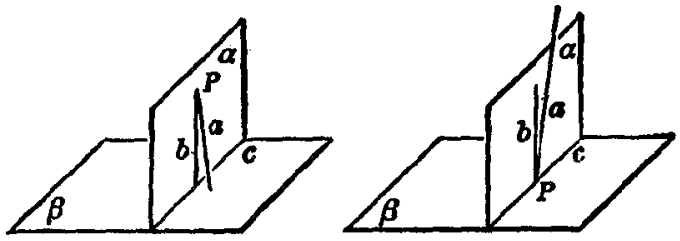
\includegraphics[width=9cm]{../pic/ltjh-ch1-51.png}
    \caption{}\label{fig:ltjh-1-51}
\end{figure}

求证: $a \subset \alpha$。

证明:设 $\alpha \cap \beta = c$。 过点 $P$ 在平面 $\alpha$ 内作直线 $b \perp c$,
根据上面的\hyperref[dl:lgpmcz-xz]{定理}有 $b \perp \beta$。

因为\hyperref[d-zx-pm]{经过一点只能有一条直线与平面 $\beta$ 垂直},所以直线 $a$ 应与直线 $b$ 重合。

即 \quad $a \subset \alpha$。


\liti 已知两条异面直线 $a$、$b$ 所成的角为 $\theta$,它们的公垂线段 $AA'$ 的长度为 $d$。
在直线 $a$、$b$ 上分别取点 $E$、$F$,设 $A'E = m$, $AF = n$,求 $EF$。

\jie 设经过 $b$ 与 $a$ 平行的平面为 $\alpha$,经过 $a$ 和 $AA'$ 的平面为 $\beta$,
$\alpha \cap \beta = c$,则 \hyperref[dl:zxhpmpx-xz]{$c \pingxing a$}。
因而 $b$、$c$ 所成的角等于 $\theta$,
且 $AA' \perp c$(图 \ref{fig:ltjh-1-52})。

又 $\because$ \quad $AA' \perp b$,

$\therefore$ \quad \hyperref[dl:zxhpmcz-pd]{$AA' \perp \alpha$}。

根据\hyperref[dl:lgpmcz-pd]{两个平面垂直的判定定理},$\beta \perp \alpha$。
在平面 $\beta$ 内作 $EG \perp c$,则 $EG = AA'$。
并且根据\hyperref[dl:lgpmcz-xz]{两个平面垂直的性质定理}, $EG \perp \alpha$。
连结 $FG$,则 $EG \perp FG$。 在直角三角形 $FEG$ 中,
$$ EF^2 = EG^2 + FG^2 \juhao $$

$\because$ \quad $AG = m$,

$\therefore$ \quad 在 $\triangle AFG$ 中,
$$ FG^2 = m^2 + n^2 - 2mn \cos\theta \juhao \footnote{录注:余弦定理。详见初中代数《第四册》。} $$

又 $\because$ \quad $EG^2 =d^2$,

$\therefore$ \quad $EF^2 = d^2 + m^2 + n^2 - 2mn\cos\theta \juhao $

如果点 $F$(或$E$)在点 $A$(或$A'$)的另一侧,则
$$ EF^2 = d^2 + m^2 + n^2 + 2mn\cos\theta \juhao $$

因此,\zhongdian{$\bm{EF = \sqrt{d^2 + m^2 + n^2 \pm 2mn\cos\theta}}$。}


在上例中,我们注意到,$AA' = EG$。 它们都是平面 $\alpha$ 的垂线,而 $EF$ 是斜线,$AA' < EF$。
所以,两条异面直线的距离,是分别在两条异面直线上的两点间的距离中最小的。

在实际中,两条交叉的高压电线如果放电时,火花正是通过它们的最短距离。

\begin{figure}[htbp]
    \centering
    \begin{minipage}[b]{7cm}
        \centering
        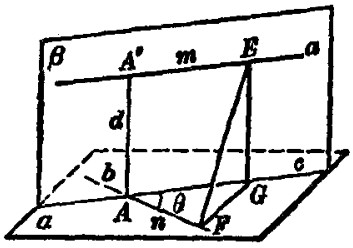
\includegraphics[width=6cm]{../pic/ltjh-ch1-52.png}
        \caption{}\label{fig:ltjh-1-52}
    \end{minipage}
    \qquad
    \begin{minipage}[b]{7cm}
        \centering
        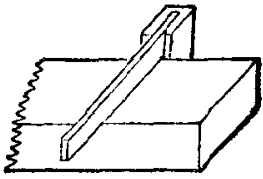
\includegraphics[width=4cm]{../pic/ltjh-ch1-subsec15-lx-02.png}
        \caption*{(第 2 题)}
    \end{minipage}
\end{figure}


\begin{lianxi}

\xiaoti{画互相垂直的两个平面、两两垂直的三个平面。}

\xiaoti{如图,检查工件的相邻两个面是否垂直时,只要用曲尺的一边紧靠在工件的一个面上,
    另一边在工件的另一个面上转动一下,观察尺边是否和这个面密合就可以了。为什么?如果不转动呢?
}

\xiaoti{在 $60^\circ$ 二面角的棱上,有两个点 $A$、$B$, $AC$、$BD$ 分别是在这个二面角的两个面内垂直于AB的线段。
    已知:$AB = 4$ cm, $AC = 6$ cm, $BD = 8$ cm。利用异面直线上两点间距离公式求 $CD$。
}

\end{lianxi}

